\chapter{Lie theory and Jacobi diagrams}
\label{ch:lie-theory-and-jacobi-diagrams}

The fundamental theorem of Vassiliev invariants states that the bialgebra of Vassiliev invariants can be broken up into nice combinatiorial weight systems. So to understand \(\mathcal{V}\) it suffices to understand \(\mathcal{W}\), or equivalently its dual \(\mathcal{A}\). There is a hint that the structure of \(\mathcal{A}\) may relate to Lie algebras.

% TODO: Try to fix(?) and include the below CDM proof of Milnor-Moore. Update: The (elusive) full proof is in Lescop 2024!

\section{Jacobi diagrams, AS, STU and IHX}

This side of the story reframes the bialgebra \(\mathcal{A}\) as an isomorphic bialgebra known as the algebra of Jacobi diagrams to illuminate the Lie theory connections.

\begin{definition}
	A \textbf{unitrivalent diagram} is a unitrivalent graph (with loops and multiple edges allowed) with the following additional data:
	\begin{itemize}
		\item each trivalent vertex has a fixed cyclic order of incident edge-connections,
		\item the set of univalent vertices has a fixed cyclic order.
	\end{itemize}
	The vector space of unitrivalent diagrams is denoted \(\mathcal{T}\).
\end{definition}

When drawing unitrivalent diagrams, there are two notation conventions. Firstly, the fixed cyclic order of the univalent edges of is specified by drawing them connected to a circle (the cyclic order is induced by traversing the circle anticlockwise).  Secondly, all the trivalent vertices are taken with the anticlockwise cyclic ordering unless an arrow around that vertex indicates otherwise.

In particular, from the first point, all chord diagrams are unitrivalent diagrams with only univalent vertices (the chord ends). Further examples of unitrivalent diagrams would be
\[
	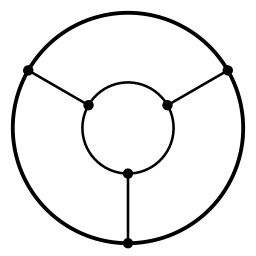
\includegraphics[width=0.13\textwidth, valign=c]{graphics/unitrivalent_diagram_example_1.pdf} \ ,
	\quad
	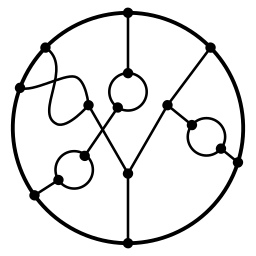
\includegraphics[width=0.13\textwidth, valign=c]{graphics/unitrivalent_diagram_example_2.pdf}
	\in \mathcal{T}.
\]

\begin{definition}
	The \textbf{STU relation} is the relation
		\begin{equation}
			\label{eq:STU}
			\tag{\stu}
			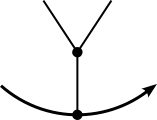
\includegraphics[width=0.10\textwidth, valign=c]{graphics/stu_relation_s.pdf}
			\quad
			=
			\quad
			\includegraphics[width=0.10\textwidth, valign=c]{graphics/stu_relation_t.pdf}
			\quad
			-
			\quad
			\includegraphics[width=0.10\textwidth, valign=c]{graphics/stu_relation_u.pdf}.
		\end{equation}
\end{definition}

As usual, this is not an individual relation but a type of relations, true in any diagrams that are identical except for the subdiagrams being as shown.

Note that the for the chord diagrams inside the algebra of Jacobi diagrams, the \ref{eq:STU} relations imply the \ref{eq:4T} relations, as
	\[
		\adjustbox{valign=c}{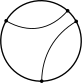
\includegraphics[width=0.115\textwidth]{graphics/four_term_from_stu_north.pdf}}
		\ - \
		\adjustbox{valign=c}{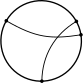
\includegraphics[width=0.115\textwidth]{graphics/four_term_from_stu_south.pdf}}
		\ = \
		\adjustbox{valign=c}{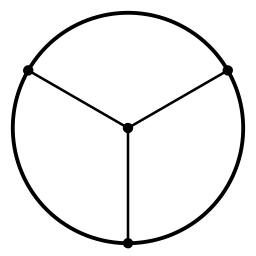
\includegraphics[width=0.12\textwidth]{four_term_jacobi_diagram.pdf}}
		\ = \
		\adjustbox{valign=c}{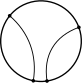
\includegraphics[width=0.115\textwidth]{graphics/four_term_from_stu_west.pdf}}
		\ - \
		\adjustbox{valign=c}{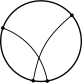
\includegraphics[width=0.115\textwidth]{graphics/four_term_from_stu_east.pdf}}\ .
	\]

\begin{definition}
	The algebra \(\mathcal{J}\) of Jacobi diagrams is the vector space \(\mathcal{T} / \ref{eq:STU}\), with the product \(\connect\) defined the same way as it was for chord diagrams.
\end{definition}

This is well-defined. The proof of Proposition \ref{prop:connected-sum-well-defined} showed that the product \(\connect\) being well-defined on \(\mathcal{A}\) was a consequence of the \ref{eq:4T} relations, which are implied by the \ref{eq:STU} relations. From the \ref{eq:STU} relations, we may deduce the following other relations which hold in \(\mathcal{J}\).

\begin{proposition}
	The following relations are consequences of the \textup{\ref{eq:STU}} relation in \(\mathcal{J}\):
	\begin{enumerate}
		\item The \textbf{AS relation} (antisymmetry relation),
			\begin{equation}
				\label{eq:AS}
				\tag{\as}
				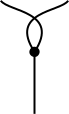
\includegraphics[width=0.05\textwidth, valign=c]{graphics/as_relation_a.pdf}
				\quad
				=
				\quad
				-
				\includegraphics[width=0.05\textwidth, valign=c]{graphics/as_relation_s.pdf}.
			\end{equation}
		\item The \textbf{IHX relation},
			\begin{equation}
				\label{eq:IHX}
				\tag{\ihx}
				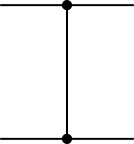
\includegraphics[width=0.10\textwidth, valign=c]{graphics/ihx_relation_i.pdf}
				\quad
				=
				\quad
				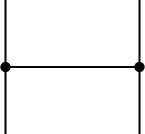
\includegraphics[width=0.10\textwidth, valign=c]{graphics/ihx_relation_h.pdf}
				\quad
				-
				\quad
				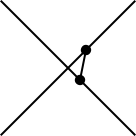
\includegraphics[width=0.10\textwidth, valign=c]{graphics/ihx_relation_x.pdf}.
			\end{equation}
	\end{enumerate}
\end{proposition}

\begin{proof}
	% TODO: Maybe put some images here.
	\begin{enumerate}
		\item
			Take two diagrams which differ only by \ref{eq:AS} at one (trivalent) vertex. If the vertex at which the \ref{eq:AS} relation resides is adjacent to a univalent vertex (i.e. touches the outer circle), then this is immediate from applying \ref{eq:STU} to both diagrams at that vertex.

			If the vertex is not immediately adjacent to a univalent vertex, then it is some \(d\) vertices `in the way'. By applying \ref{eq:STU} to those vertices yields a sum of \(2^{d}\) diagrams, all identical except for differing by \ref{eq:AS}, now on a vertex adjacent to a univalent vertex.

		\item
			A similar argument applies. If one of the two vertices of the \ref{eq:IHX} is adjacent to the circle, then the result is a direct consequence of an \ref{eq:STU} on each of the vertices. Otherwise, some \ref{eq:STU}s may be required first.
\end{enumerate}
\end{proof}

\begin{lemma}[Generalised \ref{eq:IHX}]
	The following holds in \(\mathcal{J}\) for any subgraph consisting of trivalent vertices that can be inserted into the grey box.
	\[
		\sum_{i = 0}^{m}\
		\def\svgscale{0.3}
		\raisebox{-34pt}{\input{graphics/generalised_ihx_left.pdf_tex}}
		\quad
		=
		\quad
		\sum_{i = 0}^{n}\
		\def\svgscale{0.3}
		\raisebox{-34pt}{\input{graphics/generalised_ihx_right.pdf_tex}}
	\]
\end{lemma}

The result is standard, see Chapter 5.2 of \cite{introduction-to-vassiliev-invariants} for a proof.
% TODO: Maybe I want to prove this.

% TODO: The change of basis assumption here is a liiitle sus.
We have already spoiled the surprise that in the end, \(\mathcal{A}\) and \(\mathcal{J}\) will be isomorphic as bialgebras. In fact, as algebras, this is clearly true so far, as \(\mathcal{J}\) is just a change of basis from \(\mathcal{A}\). Since \(\mathcal{A}\) spans \(\mathcal{J}\), we can attempt to lift the coproduct from \(\mathcal{A}\) directly onto \(\mathcal{J}\).

\begin{proposition}
	The coproduct \(\Delta\) on \(J \in \mathcal{J}\) defined by taking a Jacobi diagram, representing it as a chord diagram via \textup{\ref{eq:STU}}, taking the coproduct in \(\mathcal{A}\), then interpreting the result as a Jacobi diagram via the inclusion of \(\mathcal{A}\) into \(\mathcal{J}\), is also given by the following formula.

	\[\Delta(J) = \sum_{C \subset S} J_{C} \otimes J_{\overline{C}},\]
	where \(S\) is the set of connected components of \(J\), and \(\overline{C} = S \smallsetminus C\).
\end{proposition}

\begin{proof}
	Note that this has the same symbolic form as the coproduct in \(\mathcal{A}\) given in Definition~\ref{def:coproduct-in-chord-diagrams}, but with chords replaced by connected components of Jacobi diagrams. However, when working in \(\mathcal{A} \subset \mathcal{J}\), there are only univalent vertices, so the connected components are exactly the chords. Since \(\mathcal{A}\) forms a basis for \(\mathcal{J}\), and the formula is linear, it extends to all of \(\mathcal{J}\).
\end{proof}

\begin{corollary}
	The primitive elements \(\mathcal{P}(\mathcal{A})\) are the connected Jacobi diagrams.
\end{corollary}

\begin{corollary}
	The bialgebras \(\mathcal{A}\) and \(\mathcal{J}\) are isomorphic.
\end{corollary}

\begin{warning}
	Justified by this isomorphism, we write \(\mathcal{J} = \mathcal{A}\), and \(\mathcal{A}\) is the preferred choice of notation for both chord diagrams and Jacobi diagrams.
\end{warning}

\section{Lie algebra weight systems}
Similar diagrammatic relations to \ref{eq:STU}, \ref{eq:AS} and \ref{eq:IHX} satisfied by \(\mathcal{A}\) are appear also in the context of a graphical notation for multilinear maps, a fact which we may exploit to probe \(\mathcal{A}\). Before seeing how, let us review this graphical notation following \cite{wheeling-a-diagrammatic-analogue-of-the-duflo-isomorphism, on-the-rozansky-witten-weight-systems}.

\begin{remark}
	This diagrammatic calculus is well-known but it goes by many names: string diagram calculus, Penrose calculus, tensor calculus, diagrammatic calculus for tensors, etc. We call them string diagrams.
\end{remark}

A tensor is a multilinear map \(X_{1} \otimes X_{2} \otimes \cdots \otimes X_{n} \to Y_{1} \otimes Y_{2} \otimes \cdots \otimes Y_{m}\), or equivalently (via the classical canonical isomorphism) an element of the vector space \(X_{1}^{\ast} \otimes X_{2}^{\ast} \otimes \cdots X_{n}^{\ast} \otimes Y_{1} \otimes Y_{2} \otimes \cdots \otimes Y_{m}\).

A tensor can be represented as a vertex with \(m + n\) unbound directed edges; \(m\) incoming edged decorated by the corresponding vector spaces (in the example above, \(X_{1}, \cdots\)), and \(n\) outgoing edges decordated by \(Y_{1}, \cdots\). For example, the bracket in a Lie algebra \(\mathfrak{g}\) is an element \([\cdot,\cdot] \in \mathfrak{g}^{\ast} \otimes \mathfrak{g}^{\ast} \otimes \mathfrak{g}\), expressed as
\[\def\svgscale{0.3} \input{graphics/bracket_string_diagram.pdf_tex}.\]
In fact, since the relation if true for any elements \(x, y \in \mathfrak{g}\), the labels on the edges can be dropped.

Such a notation is useful because composition of tensors can be expressed graphically by connecting outgoing and incoming legs with the same decoration. Relations can therefore be expressed graphically, for example, the antisymmetry of the bracket \([y, x] = -[x, y]\) becomes
\[
	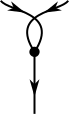
\includegraphics[width=0.05\textwidth, valign=c]{graphics/bracket_antisymmetry_swap.pdf}
	\quad
	=
	\quad
	-
	\includegraphics[width=0.05\textwidth, valign=c]{graphics/bracket_antisymmetry_id.pdf}.
\]
the Jacobi relation \([[x, y], z] + [[y, z], x] + [[z, x], y] = 0\) becomes
\[
	\includegraphics[width=0.10\textwidth, valign=c]{graphics/jacobi_symmetric_xyz.pdf}
	\quad
	+
	\quad
	\includegraphics[width=0.10\textwidth, valign=c]{graphics/jacobi_symmetric_yzx.pdf}
	\quad
	+
	\quad
	\includegraphics[width=0.10\textwidth, valign=c]{graphics/jacobi_symmetric_zxy.pdf}
	\quad
	=
	\quad
	0
\]

Looking at the relations these relations in the tensor algebra \(\mathcal{T}(\mathfrak{g})\), the first solid evidence of Lie-theoretic structure in this story emerges. The antisymmetry of the bracket, drawn as a string diagram looks like a directed version of \ref{eq:AS}. Similarly the string diagram Jacobi relation can be arranged into a directed version of \ref{eq:IHX}.

% TODO: Decide whether we can be bothered to talk about representations also as vertices. We can also just weight systems into U(g) then take traces wrt a rep after.

Furthermore, suppose \(\mathfrak{g}\) is a metric Lie algebra. Then it has an invariant, nondegenerate, bilinear form \(\langle \cdot, \cdot \rangle \in \mathfrak{g}^{\ast} \otimes \mathfrak{g}^{\ast}\). Being nondegenerate, it can be inverted to an element \(c \in \mathfrak{g} \otimes \mathfrak{g}\). We have additional bivalent vertices
\[
	\includegraphics[width=0.06\textwidth, valign=c]{graphics/string_diagram_metric.pdf}
	\qquad \text{and} \qquad
	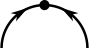
\includegraphics[width=0.06\textwidth, valign=c]{graphics/string_diagram_casimir.pdf}\ .
\]
These can be used to change the arrow direction on any edge, allowing us to drop the edge arrows from the notation.

Moreover, the invariance of the metric can be written as \(\langle [x, y], z \rangle = \langle [y, z], x \rangle\) which graphically can be represented as cyclic invariance of the contraction of the bracket and the metric
\[
	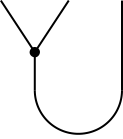
\includegraphics[width=0.08\textwidth, valign=c]{graphics/bracket_metric_cyclic_invariance_bracketxy.pdf}
	\quad
	=
	\quad
	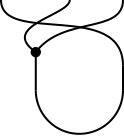
\includegraphics[width=0.08\textwidth, valign=c]{graphics/bracket_metric_cyclic_invariance_permute.pdf}
	\quad
	=
	\quad
	\includegraphics[width=0.08\textwidth, valign=c]{graphics/bracket_metric_cyclic_invariance_bracketyz.pdf}.
\]
A similar argument works for the casimir.

A representation of \(\mathfrak{g}\) into a finite-dimensional vector space \(V\) takes the form \(\rho \in \mathfrak{g}^{\ast} \otimes V^{\ast} \otimes V\). This takes a new kind of input an output, namely a \(v \in V\) which we denote by a thick line at a shallow angle
\[
	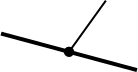
\includegraphics[width=0.11\textwidth, valign=c]{graphics/representation_vertex.pdf}.
\]
The identity the action is a Lie action, \[\rho([x, y]) = \rho(x)\rho(y) - \rho(y)\rho(x)\] is graphically
\[
	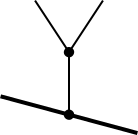
\includegraphics[width=0.1\textwidth, valign=c]{graphics/string_diagram_lie_action_s.pdf}
	\quad
	=
	\quad
	\includegraphics[width=0.1\textwidth, valign=c]{graphics/string_diagram_lie_action_t.pdf}
	\quad
	-
	\quad
	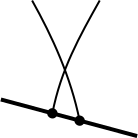
\includegraphics[width=0.1\textwidth, valign=c]{graphics/string_diagram_lie_action_u.pdf}.
\]
Again, arrows are unnecessary on the thick edges corresponding to inputs and outputs of \(V\), as cup and cap vertices similar to the metric and casimir for \(\mathfrak{g}\) are given by the maps
\[f \otimes v \longmapsto f(v) \quad \text{and} \quad 1 \longmapsto \sum_{i} e_{i} \otimes e_{i}^{\ast}.\]

The famous construction of Bar-Natan \cite{on-the-vassiliev-knot-invariants} uses this diagrammatic calculus to take metric Lie algebras and produce weight systems.

% TODO: According to Chmutov-Duzhin-Mostovoy, p164, the weight system is only multiplicative if the representation is irreducible. Question for Zsuzsi: does this mean we only get a quotient of A if we put in an irreducible representation?
\begin{theorem}
	The construction below which takes a lie algebra \(\mathfrak{g}\) produces a well-defined weight system \(W_{\mathfrak{g}}\) valued in \(\mathcal{U}(\mathfrak{g})\).
	% TODO: Should this be Q?
	Furthermore if a representation, \(\rho\) of \(\mathfrak{g}\) is given, then a \(\mathbb{C}\)-valued weight system is produced.
\end{theorem}

\begin{construction}
	\label{cons:lie-algebra-weight-system}
	Given a Lie algebra \(\mathfrak{g}\), the vertex \(m\) with signature \(\mathfrak{g} \otimes \mathfrak{g} \otimes \mathfrak{g}\) is associated to a genuine element of the tensor algebra \(T_{\mathfrak{g}}(m) \in \mathfrak{g}^{\otimes 3}\). For each trivalent vertex of the Jacobi diagram \(J \in \mathcal{A}\), take \(T_{\mathfrak{g}}(m)\), and take all of their tensor products, in arbitrary order. There being \(v\) trivalent vertices, this lies in \(\mathfrak{g}^{\otimes 3v}\).

	For each edge between the trivalent vertices in the Jacobi diagram, contract the corresponding variables in \(\mathfrak{g}^{\otimes 3 v}\). The result lies in \(\mathfrak{g}^{\otimes 3v - 2e}\) where \(e\) is the number of edges between trivalent vertices.

	The number of univalent vertices matches the number of remaining uncontracted trivalent vertices, \(u = 3v - 2e\). In-particular the edges between univalent and trivalent vertices, along with the cyclic order on univalent vertices determines a cyclic order on the remaining trivalent vertices. So, a cyclic order on the factors of \(\mathfrak{g}^{\otimes 3v - 2e} = \mathfrak{g}^{\otimes u}\). Permute the factors into an order which respects the induced cyclic order (there are many --- choose one). Projecting from the tensor algebra of \(\mathfrak{g}\) into its universal enveloping algebra, we obtain an element \(W_{\mathfrak{g}}(J) \in \mathcal{U}(\mathfrak{g})\).

	A representation \(\rho: \mathfrak{g} \to \operatorname{Hom}(V)\) of \(\mathfrak{g}\) extends uniquely to a representation \(\rho: \mathcal{U}(\mathfrak{g}) \to \operatorname{Hom}(V)\) of \(\mathcal{U}(\mathfrak{g})\). Use this representation to take the trace of \(W_{\mathfrak{g}}(J)\). The result is an element of the ground field \(W_{\mathfrak{g}, \rho}(J) = \operatorname{tr}(\rho(T_{\mathfrak{g}}(J))) \in \mathbb{C}\).
\end{construction}

\begin{warning}
	When constructing \(T_{\mathfrak{g}}(m)\), the tensor factors in the tensor corresponding to the bracket need to have the unusual cyclic order \((y, x, [x, y]_{\mathfrak{g}})\). This is because its projection into \(\mathcal{U}(\mathfrak{g})\) should obey \ref{eq:STU}, and this is the cyclic order of the trivalent vertex in \ref{eq:STU}.
\end{warning}

Hence, we have the functions \(W_{\mathfrak{g}}: \mathcal{A} \to \mathcal{U}(\mathfrak{g})\) and \(W_{\mathfrak{g}, \rho}: \mathcal{A} \to \mathbb{C}\) which we claim are weight systems.

\begin{proof}
	The contruction creates a string diagram which is well-defined modulo certain diagrammatic relations as seen at the start of this section such as the cyclic invariance of the contraction of the metric and bracket. By \cite[Proposition 3.1.1]{vassiliev-knot-invariants-and-lie-s-algebras}, string diagrams modulo these relations are exactly encoded by unitrivalent graphs with a cyclic order on trivalent vertices, and a linear order on univalent vertices.

	\begin{mdframed}
		Explicitly have diagrams for all the relations, involving the symmetry natural transformation, so that we can later say that this could not be the on-the-nose identity.
	\end{mdframed}

	Thus, to prove that the map \(W_{\mathfrak{g}}: \mathcal{A} \to \mathcal{U}(\mathfrak{g})\) is well-defined it suffices to show that the string diagrams obey the \(\ref{eq:STU}\) relations when interpreted as elements of \(\mathcal{U}(\mathfrak{g})\). If two chord diagrams differ by \ref{eq:STU}, on some univalent vertices associated with adjacent tensor factors \(y\) and \(x\), the construction gives
	\[\cdots \otimes [x, y]_{\mathfrak{g}} \otimes \cdots \qquad \text{and} \qquad (\cdots \otimes x \otimes y \otimes \cdots) - (\cdots \otimes y \otimes x \otimes \cdots),\]
	but this equality is exactly the quotient in the \(\mathcal{U}(\mathfrak{g})\).

	Indeed \ref{eq:AS} and \ref{eq:IHX} follow from \ref{eq:STU} but they are also easy to see directly. \(\ref{eq:AS}\) follows from the skew-symmetry of the vertex \(m\), being built out of the bracket, and \(\ref{eq:IHX}\) follows from the Jacobi identity in \(\mathfrak{g}\).

	Finally, a Jacobi diagram's univalent vertices only have a cyclic order. But in the construction a true order respecting that cyclic order was chosen. We should show that any order respecting the cyclic order leads to the same result. It suffices to show that the tensor is cyclically symmetric. Indeed, a stronger statement is true: anything satisfying the \ref{eq:STU} relation is cyclically symmetric. Since it is stronger, let us prove it instead for \(\mathcal{A}\).
	% TODO: Perhaps this could be moved above, to a corollary of the generalised IHX lemma. After all it is a structural theorem on A (and similar algebras).

	It is equivalent to prove that any Jacobi diagram on a long line is cyclically symmetric. Examine the operation of taking the univalent vertex (which we will here call legs) in the first position and moving it to the last position, reducing by one the positions of all other legs. This generates the cyclic group on the number of univalent vertices, so it is enough to show this operation preserves the Jacobi diagram. The \ref{eq:STU} relation gives the cost of commuting the first leg past the \(i\)th leg: the same diagram with the first leg attached to the \(i\)th leg. Thus cost commuting the first leg to the very last place is the sum over the other legs of attaching it to those legs. We will show that this cost is zero.

	We split this sum by the connected components of the \(i\)th leg. On components that don't contain the first leg, this is the sum, over legs, of the same diagram, with the first leg attached to the \(i\)th leg. This vanishes by the generalised \ref{eq:IHX}. On the component that contains the first leg, generalised \ref{eq:IHX} produces a diagram with a loop at the top, which is killed by \ref{eq:AS}.

	That \(W_{\mathfrak{g}, \rho}\) is a genuine weight system into \(\mathbb{C}\) follows from that a representation on \(\mathfrak{g}\) extends uniquely to \(\mathcal{U}(\mathfrak{g})\).
\end{proof}

\begin{mdframed}
	Confirm: This obeys all the relations of \(\mathcal{A}\), and more. Does this make it a quotient of \(\mathcal{A}\)?
\end{mdframed}

Let's look at a specific weight system for the Lie algebra \(\mathfrak{sl}_{2}\) \cite{on-the-vassiliev-knot-invariants, remarks-on-the-vassiliev-knot-invariants-coming-from-sl2}.
\begin{example}[Weight system for \({\mathfrak{sl}_{2}}\)]
	We choose as our Lie algebra \(\mathfrak{sl}_{2}\), generated by \(h\), \(e\) and \(f\) with commutators
	\[[h, e] = 2e, \quad [h, f] = -2f, \quad [e, f] = h.\]
	The unique invariant bilinear form up to scalar multiple is
	\[\langle h, h \rangle = 1, \quad \langle e, f \rangle = \frac{1}{2}, \quad \langle f, e \rangle = \frac{1}{2},\]
	and all other inner products are zero.

	In \cite{remarks-on-the-vassiliev-knot-invariants-coming-from-sl2}, the following skein relation is derived:
	\[
		W_{\mathfrak{sl}_{2}}
		\left(
			\includegraphics[width=0.115\textwidth, valign=c]{graphics/sl2_skein_relation_h.pdf}
		\right)
		=
		4 W_{\mathfrak{sl}_{2}}
		\left(
			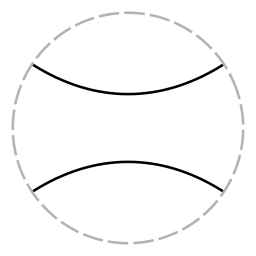
\includegraphics[width=0.115\textwidth, valign=c]{graphics/sl2_skein_relation_uu.pdf}
		\right)
		-
		4 W_{\mathfrak{sl}_{2}}
		\left(
			\includegraphics[width=0.115\textwidth, valign=c]{graphics/sl2_skein_relation_x.pdf}
		\right)
	\]

	\begin{proof}
		Associated to the Penrose diagram for each side of the above equation (it is not advisable to compute by hand) we find the tensors
		\begin{align*}
			{}- 8 h\otimes e\otimes h\otimes f && {}+ 8 & h\otimes e\otimes f\otimes h & {}- \phantom{1}8  & h\otimes f\otimes h\otimes e & {}+ \phantom{1}8  & h\otimes f\otimes e\otimes h \\
			{}+ 8 e\otimes h\otimes h\otimes f && {}- 8 & e\otimes h\otimes f\otimes h & {}+            16 & e\otimes f\otimes e\otimes f & {}-            16 & e\otimes f\otimes f\otimes e \\
			{}+ 8 f\otimes h\otimes h\otimes e && {}- 8 & f\otimes h\otimes e\otimes h & {}-            16 & f\otimes e\otimes e\otimes f & {}+            16 & f\otimes e\otimes f\otimes e
		\end{align*}
		and
		\begin{align*}
			{}+ 8 h\otimes h\otimes e\otimes f && {}+ \phantom{1}8  & h\otimes h\otimes f\otimes e & {}- \phantom{1}8  & h\otimes e\otimes h\otimes f & {}- \phantom{1}8  & h\otimes f\otimes h\otimes e \\
			{}- 8 e\otimes h\otimes f\otimes h && {}- 16 & e\otimes e\otimes f\otimes f & {}+ \phantom{1}8  & e\otimes f\otimes h\otimes h & {}+ 16 & e\otimes f\otimes e\otimes f \\
			{}- 8 f\otimes h\otimes e\otimes h && {}+ \phantom{1}8  & f\otimes e\otimes h\otimes h & {}+ 16 & f\otimes e\otimes f\otimes e & {}- 16 & f\otimes f\otimes e\otimes e.
		\end{align*}
		Projecting into \(\mathcal{U}(\mathfrak{g})\) and using one's favourite CAS to express both expressions in the Poincare-Birkhoff-Witt basis, we find both equal to
		\[64 e \otimes f + 16 h \otimes h - 32 h.\]
	\end{proof}

	\begin{mdframed}
		In fact, this skein relation is an analogue of the vector triple product rule for the cross product in \(\mathbb{R}^{3}\), which is related to the Lie algebra \(\mathfrak{sl}_{2}\) \cite{introduction-to-vassiliev-invariants}. It has been further studied in \cite{riordan-trees-and-the-homotopy-sl2-weight-system}. There is also a cross product in \(\mathbb{R}^{7}\), related to the exceptional Lie algebra \(\mathfrak{g}_{2}\). However it does not obey the vector triple product rule.
	\end{mdframed}
\end{example}
\begin{question}
	What skein relation in \(\mathcal{A}\) does the weight system for the exceptional Lie algebra \(\mathfrak{g}_{2}\) obey?
\end{question}
% TODO: Insert result here.

Bar-Natan's construction yields a way of extracting some information from \(\mathcal{A}\) by plugging in a metric Lie algebra -- doing so constructs some quotient of \(\mathcal{A}\). This naturally begs the question whether every all the information in \(\mathcal{A}\) can be extracted with some metric Lie algebra.

Computer enumeration of chord diagrams \cite{on-the-vassiliev-knot-invariants} prove this for order \(m \leq 9\), the order to which the dimensions \(\operatorname{dim}\mathcal{A}_{m} = \operatorname{dim}\mathcal{W}_{m}\) were known:
\[
	\begin{tblr}{hlines, vlines}
		m									& 0 & 1 & 2 & 3 & 4 & 5  & 6  & 7  & 8  & 9   \\ \hline % & 10  & 11  & 12  \\
		\operatorname{dim}\mathcal{A}_{m}					& 1 & 1 & 2 & 3 & 6 & 10 & 19 & 33 & 60 & 104 \\ % & 184 & 316 & 548 \\
		\operatorname{dim}(\operatorname{span}(W_{\{\mathfrak{g}, \rho\}}))	& 1 & 1 & 2 & 3 & 6 & 10 & 19 & 33 & 60 & 104 \\
	\end{tblr}
\]
Here \(\operatorname{span}(W_{\{\mathfrak{g}, \rho\}})\) denotes the dimension of the subspace of \(\mathcal{W}_{m}\) spanned by weight systems coming from Costruction \ref{cons:lie-algebra-weight-system} on representations of classical Lie algebras \(\mathfrak{sl}_{n}\) and \(\mathfrak{gl}_{n}\).

\begin{conjecture}[Bar-Natan]
	\label{conj:lie-algebra-weight-systems-span}
	All weight systems are obtained as Lie algebra weight systems. In other words the set \(\{W_{\mathfrak{g}, \rho} \,|\, \text{\(\mathfrak{g}\) a Lie algebra}, \text{\(\rho\) a representation of \(\mathfrak{g}\)}\}\) spans \(\mathcal{W}\).
\end{conjecture}

\begin{remark}
	\label{rem:chord-diagram-universal-construction}
	Strenthening the above conjecture, maybe even there is some universal Lie algebra, applying the construction to which, recovers exactly \(\mathcal{A}\), losing no information.
\end{remark}

\section{Non-Lie algebraic weight systems}
\label{sec:non-lie-algebraic-weight-systems}

Quite surprisingly, Conjecture \ref{conj:lie-algebra-weight-systems-span} is false. This may be a surprise to the reader: the relation \([x, y] = x y - y x\) in the universal enveloping algebra of a Lie algebra looks like it encodes exactly the \ref{eq:STU} relation in \(\mathcal{A}\). But the Conjecture being false implies that weight systems coming from Lie algebras are just a specific kind.

In fact, \ref{eq:STU} is more general than \([x, y] = xy - yx\), and Construction \ref{cons:lie-algebra-weight-system} is just one example of a more general construction introduced by Vogel and Vaintrob to construct weight systems coming from metric Lie super-algebras. The most general type of objects these constructions apply to are called by Vaintrob \cite{vassiliev-knot-invariants-and-lie-s-algebras} `Lie \(S\)-algebras', but we will follow the more modern approach of \cite{on-the-rozansky-witten-weight-systems, rozansky-witten-theory} and they will be known as Lie algebra objects in a symmetric monoidal category. They are related to Vogel's ``Universal Lie algebra'' construction, \cite{vassiliev-theory-and-the-universal-lie-algebra}, and also related to the structures studied in \cite{cyclic-operads-and-the-algebra-of-chord-diagrams}. First, we need the following category-theoretic notions.

\begin{definition}
	A (\textbf{weak}) \textbf{monoidal category} is a category \(\mathcal{C}\) equipped with a functor
	\[
		\begin{array}{rccc}
			\otimes:	&\mathcal{C} \times \mathcal{C}		&\longrightarrow	&\mathcal{C}\\
					&(A, B)					&\longmapsto		&A \otimes B,
		\end{array}
	\]
	an \textbf{unit} object \(k \in \mathcal{C}\), and natural isomorphisms
	\[
		 \otimes \circ (\otimes \times \operatorname{id}) \longrightarrow \otimes \circ (\operatorname{id} \times \otimes)  \quad \text{ and }\ \quad  \otimes \longrightarrow \operatorname{id}
	\]
	satisfying some relations known as the pentagon and triangle relations. The natural isomorphisms give isomorphisms
	\[(A \otimes B) \otimes C \cong A \otimes (B \otimes C), \qquad k \otimes A \cong A \cong A \otimes k\]
	for every tuple of objects \(A, B\) and \(C\) in \(\mathcal{C}\). If these isomorphisms are equalities, then \(\mathcal{C}\) is a \textbf{strict} monoidal category.
\end{definition}

\begin{remark}
	\label{rem:coherence-for-monoidal-categories}
	Omitting the details, we assume that these natural isomorphisms are equalities, for example that \((A \otimes B) \otimes C = A \otimes (B \otimes C)\). This is acceptable by the coherence theorem for monoidal categories which says that every monoidal category is equivalent to a strict monoidal category, and it's why we omit the pentagon and triangle relations in the definition above. We refer to \cite{higher-operads-higher-categories} for details.
\end{remark}

\begin{definitions}
	\begin{enumerate}
		\item The \textbf{flip functor} is the functor
			\[
				\begin{array}{rccc}
					\sigma:		&\mathcal{C} \times \mathcal{C}		&\longrightarrow	&\mathcal{C} \times \mathcal{C}\\
						&(A, B)					&\longmapsto		&(B, A).
				\end{array}
			\]

		\item A \textbf{symmetric monoidal category} is a monoidal category \(\mathcal{C}\) equipped with a \textbf{symmetry natural isomorphism} \(\tau\)
			\[\otimes \longrightarrow \otimes \circ \sigma\]
			satisfying the hexagon relation. The \textbf{hexagon relation} is the relation that the isomorphisms
			\[
				\tau_{A, B}: A \otimes B \overset{\cong}{\longrightarrow} B \otimes A
			\]
			coming from the natural isomorphism \(\tau\) obey
			% TODO: Fix A,A below
			\[\tau_{A, B \otimes C} = (\operatorname{id}_{B} \mathbin{\otimes} \tau_{A, A}) \circ (\tau_{A, B} \mathbin{\otimes} \operatorname{id}_{C})\]
			for every pair of objects \(A\), and \(B\) in \(\mathcal{C}\).
	\end{enumerate}
\end{definitions}
The hexagon relations have six terms instead of three when the associators omitted due to Remark \ref{rem:coherence-for-monoidal-categories} are reintroduced.

If the tensor category is additionally additive, we can define the following.

\begin{definitions}
	\begin{enumerate}
		\item A \textbf{Lie algebra object} in an additive symmetric tensor category \(\mathcal{C}\) is an object \(L\) equipped with a bracket morphism \(\beta\) such that
			\[\left( \beta \circ (\beta \otimes \operatorname{id}) \right) \circ (1 + \tau_{123} + (\tau_{123})^{2}) = 0 \qquad \text{and} \qquad \beta + \beta \circ \tau = 0.\]
			Graphically, in terms of the string diagrams of the previous section, this is
			\[
				\def\svgscale{0.31}
				\adjustbox{valign=c}{\input{graphics/jacobi_symmetric_arbitrary_monoidal_cat_xyz.pdf_tex}}
				\quad
				+
				\quad
				\def\svgscale{0.31}
				\adjustbox{valign=c}{\input{graphics/jacobi_symmetric_arbitrary_monoidal_cat_yzx.pdf_tex}}
				\quad
				+
				\quad
				\def\svgscale{0.31}
				\adjustbox{valign=c}{\input{graphics/jacobi_symmetric_arbitrary_monoidal_cat_zxy.pdf_tex}}
				\quad
				=
				\quad
				0,
			\]
			\[
				\def\svgscale{0.35}
				\adjustbox{valign=c}{\input{graphics/bracket_antisymmetry_arb_mon_cat_id.pdf_tex}}
				\quad
				+
				\quad
				\def\svgscale{0.35}
				\adjustbox{valign=c}{\input{graphics/bracket_antisymmetry_arb_mon_cat_swap.pdf_tex}}
				\quad
				=
				\quad
				0.
			\]
		\item A \textbf{representation of a Lie algebra object} \(L\) in \(\mathcal{C}\) into an object \(V\) in \(\mathcal{C}\) is a morphism \(\rho: L \otimes V \to V\), such that
			\[
				\def\svgscale{0.31}
				\adjustbox{valign=c}{\input{graphics/string_diagram_lie_action_arb_mon_cat_s.pdf_tex}}
				\quad
				=
				\quad
				\def\svgscale{0.31}
				\adjustbox{valign=c}{\input{graphics/string_diagram_lie_action_arb_mon_cat_t.pdf_tex}}
				\quad
				-
				\quad
				\def\svgscale{0.31}
				\adjustbox{valign=c}{\input{graphics/string_diagram_lie_action_arb_mon_cat_u.pdf_tex}}
				.
			\]
		\item A \textbf{metric Lie algebra object} \(L\) in \(\mathcal{C}\) is a Lie algebra object in \(\mathcal{C}\), further equipped with the following modules over \(L\)...
	\end{enumerate}
\end{definitions}


We will give various concrete examples of Lie algebra objects in different symmetric tensor categories later. But for now, let's show that this data can still be used to construct weight systems, generalising Construction \ref{cons:lie-algebra-weight-system}.

\begin{theorem}[\cite{ vassiliev-knot-invariants-and-lie-s-algebras}]
	% TODO: Check that all the ajectives have been defined, or at least thought about.
	Let \(\mathcal{C}\) be a rigid, additive, symmetric monoidal category, \(L\) a metric Lie algebra in \(\mathcal{C}\), and \(M\) a dualisable representation \(\eta\). Then, there is a weight system
	\[W_{L, \eta}: \mathcal{A} \longrightarrow \mathcal{C}(k, k) \cong k.\]
\end{theorem}
\begin{proof}
	Similar to the proof of the construction...
\end{proof}

The difference between this construction and Bar-Natan's original one is the treatment of the symmetry natural isomorphism \(\tau\). This tells us which isomorphism to use when rearranging the tensor factors. The most obvious isomorphism would be the identity, as it was in the original construction, corresponding to when \(\mathcal{C}\) is a strict symmetric (strict) monoidal category. However unlike for general monoidal categories, not every symmetric monoidal category is equivalent to a strict symmetric monoidal category. At a down-to-earth level, Lie algebra objects with non-trivial symmetry isomorphisms are necessary to pick up all the structure in \(\mathcal{A}\).

\begin{example}
	If we take \(\mathcal{C} = \mathbf{sVect}\), the symmetric monoidal category of super vector spaces, the Lie algebra objects are the following.

	A \textbf{Lie superalgebra} \(\mathfrak{g}\) is a vector space with a \(\mathbb{Z} / 2\mathbb{Z}\) grading, equipped with a bracket \([\cdot,\cdot]: \mathfrak{g} \otimes \mathfrak{g} \to \mathfrak{g}\) satisfying some axioms to follow. The grading induces the splitting \(\mathfrak{g} = \mathfrak{g}_{0} \oplus \mathfrak{g}_{1}\), and the direct summand \(\mathfrak{g}_{0}\) is known as the \textbf{even} part and the summand \(\mathfrak{g}_{1}\) is known as the \textbf{odd} part.

	The axioms a Lie superalgebra must satisfy are the following analogues of the usual lie algebra axioms. Let \(x, y, z\) be homogeneous elements, so in \(\mathfrak{g}_{i}, \mathfrak{g}_{j}\), and \(\mathfrak{g}_{k}\) respectively, then \textbf{super symmetry} axiom is
		\[[x, y] = - (-1)^{ij}[y, x],\]
		and the \textbf{super Jacobi identity} is the axiom
		\[(-1)^{ik}[x, [y, z]] + (-1)^{ji}[y, [z, x]] + (-1)^{kj}[z, [x, y]] = 0.\]
\end{example}

Shortly after Conjecture \ref{conj:lie-algebra-weight-systems-span} was made, the following results were achieved based on constructions with the exceptional Lie superalgebra \(\mathfrak{D}(2, 1; \alpha)\).

\begin{theorem}
	There are primitive Jacobi diagrams of order at least 17 \cite{algebraic-structures-on-modules-of-diagrams-preprint} and at least 15 \cite{on-vassiliev-invariants-not-coming-from-semisimple-lie-algebras} which vanish on all Lie algebra weight systems. 
\end{theorem}

Furthermore, as was known about shortly after but not published until significantly later,
\begin{theorem}
Vogel's diagram of order 17 vanishes also on all Lie superalgebra weight systems \cite{algebraic-structures-on-modules-of-diagrams}.
\end{theorem}

\begin{corollary}
	The set of Lie (super-) algebra weight systems does not span \(\mathcal{W}\).
\end{corollary}

In general, it is still unknown to what exact level of generality one needs to go (what type of symmetric monoidal categories need to be considered) in order to generate all weight systems.

Roberts and Willerton in \cite{rozansky-witten-theory} and \cite{on-the-rozansky-witten-weight-systems} examine weight systems constructructed from Lie algebra objects in the derived category of complex manifolds. Such weight systems are candidates for being able to detect knot orientation, which Lie algebra weight systems cannot \cite{on-the-vassiliev-knot-invariants}. However, computing these weight systems is difficult, and to our knowledge, no computations exist in the literature.

More recently Aizawa-Kimura \cite{universal-weight-systems-from-a-mimimal-Z22-graded-lie-algebra}, have conducted some preliminary investigations into the class of colour Lie algebras (also known as \(\epsilon-\)Lie algebras). This class generalises the \(\mathbb{Z}/2\mathbb{Z}\) grading on Lie superalgebras to a more general type of group and sign rule. Their example lies within the span of the \(\mathfrak{sl}_{2}\) and \(\mathfrak{gl}_{1 | 1}\) weight systems.

\section{A universal metric Lie algebra object}

There is however a theoretical construction of Hinnich-Vaintrob \cite{cyclic-operads-and-the-algebra-of-chord-diagrams} which provides the moral version of the statement in Remark \ref{rem:chord-diagram-universal-construction}. They construct a Lie algebra object in a symmetric tensor category whose weight system (in a certain sense) is isomorphic to \(\mathcal{A}\). Note, however that the objects in this category are not sets, but simply objects, so the result is theoretically rather than computationally useful.
